% 图 60.3 —— 由 `checks/emit_hand.py` 自动拼出（probe 精测 + prims2 图元分解）
%%
% ⚠ 这是**稿子不是成品**：跑 `checks/checkhand.py 60.3` 看指标 + 看叠合图。
%%
%% ⚠ 待核：
%   · 本图 probe 报出阴影族 1 个 —— **本脚本不生成阴影**（要照原书手写）；prims2 的 strokes 里可能含阴影线，核对时留意别画重
%   · 可疑字形 1 项（空心圈 ⊙ 常被认成字母 o）—— 见文件末
%%
\documentclass[12pt]{standalone}
\usepackage{fontspec}
\setsansfont{Arial}
\newfontfamily\mfallback{DejaVu Sans}
\usepackage{tikz}
\begin{document}
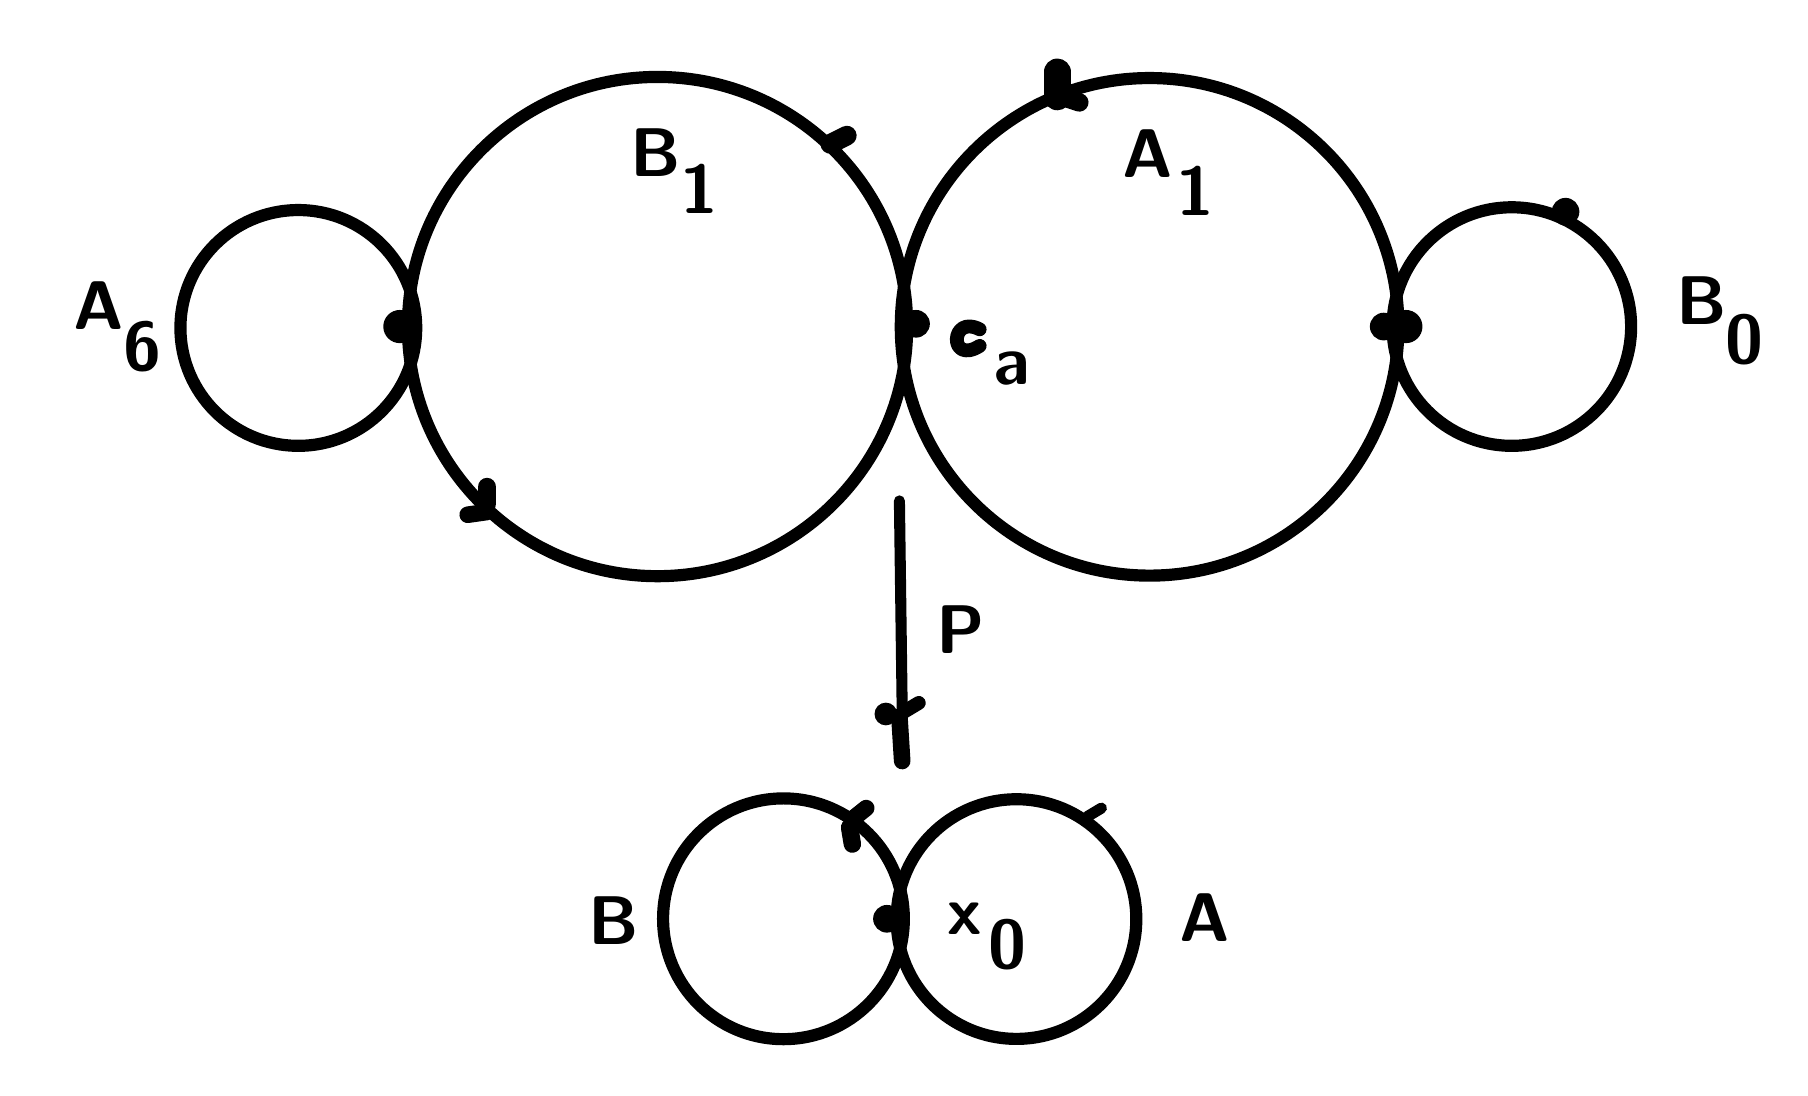
\begin{tikzpicture}[x=1pt, y=-1pt, line width=4.4pt, line cap=round, line join=round]

  %% ════ 填充区（prims2 的 fills）════

  %% ════ 直线段（prims2 的 strokes）════
  \draw[line width=6.3pt] (297.0,289.0) -- (298.0,295.0);
  \draw[line width=6.0pt] (298.0,286.0) -- (303.0,282.0);
  \draw[line width=6.7pt] (166.0,172.0) -- (166.0,166.0);
  \draw[line width=9.7pt] (372.0,25.0) -- (372.0,16.0);
  \draw[line width=7.1pt] (290.0,42.0) -- (296.0,39.0);
  \draw[line width=6.7pt] (374.0,25.0) -- (380.0,27.0);
  \draw[line width=6.0pt] (315.0,249.0) -- (316.0,265.0);
  \draw[line width=4.0pt] (383.0,285.0) -- (388.0,282.0);
  \draw[line width=6.0pt] (159.0,176.0) -- (166.0,175.0);
  \draw[line width=4.0pt] (316.0,246.0) -- (315.0,171.0);
  \draw[line width=5.0pt] (317.0,247.0) -- (322.0,244.0);

  %% ════ 曲线（prims2 的 curves —— 三段式，坐标同为 (y,x)）════
  \draw[line width=5.0pt] (344.0,109.0) .. controls (333.3,103.4) and (332.7,122.1) .. (344.0,115.0);

  %% ════ 圆 / 椭圆（probe 精测）════
  \draw (227.6,108.0) circle (90.2);
  \draw (405.4,108.1) circle (89.9);
  \draw (357.3,322.1) circle (43.3);
  \draw (97.8,108.5) circle (42.6);
  \draw (536.3,108.0) circle (43.1);
  \draw (273.1,322.0) circle (43.5);

  %% ════ 实心点 ════
  \fill (555.7,66.5) circle (5.0);
  \fill (134.5,108.0) circle (6.0);
  \fill (321.0,107.0) circle (5.0);
  \fill (490.0,108.0) circle (5.0);
  \fill (498.0,108.0) circle (6.0);
  \fill (310.1,248.0) circle (4.1);
  \fill (310.5,322.0) circle (5.0);

  %% ════ 标签（probe 直接给的 \node 行）════
  %% ⚠ 全部补了 fill=white：文字在最上层，否则与曲线交叉干扰
     \node[anchor=center,inner sep=0pt,fill=white,font=\fontsize{31.0}{38.8}\selectfont] at (226.8,45.0) {\textsf{\textbf{\textit{B}}}};   % box(215,33,20,23)
     \node[anchor=center,inner sep=0pt,fill=white,font=\fontsize{30.3}{37.9}\selectfont] at (404.8,45.5) {\textsf{\textbf{\textit{A}}}};   % box(392,34,20,22)
     \node[anchor=center,inner sep=0pt,fill=white,font=\fontsize{23.7}{29.7}\selectfont] at (242.8,58.4) {\textsf{\textbf{1}}};   % box(236,50,8,16)
     \node[anchor=center,inner sep=0pt,fill=white,font=\fontsize{23.7}{29.7}\selectfont] at (421.8,59.4) {\textsf{\textbf{1}}};   % box(415,51,8,16)
     \node[anchor=center,inner sep=0pt,fill=white,font=\fontsize{30.3}{37.9}\selectfont] at (604.8,98.5) {\textsf{\textbf{\textit{B}}}};   % box(593,87,20,22)
     \node[anchor=center,inner sep=0pt,fill=white,font=\fontsize{30.3}{37.9}\selectfont] at (25.8,100.5) {\textsf{\textbf{\textit{A}}}};   % box(13,89,20,22)
     \node[anchor=center,inner sep=0pt,fill=white,font=\fontsize{23.8}{29.8}\selectfont] at (620.5,112.7) {\textsf{\textbf{0}}};   % box(613,104,11,17)
     \node[anchor=center,inner sep=0pt,fill=white,font=\fontsize{24.4}{30.5}\selectfont] at (41.6,115.1) {\textsf{\textbf{6}}};   % box(35,106,12,17)
     \node[anchor=center,inner sep=0pt,fill=white,font=\fontsize{26.9}{33.6}\selectfont] at (355.9,123.3) {\textsf{\textbf{\textit{a}}}};   % box(349,114,12,16)
     \node[anchor=center,inner sep=0pt,fill=white,font=\fontsize{29.8}{37.3}\selectfont] at (337.0,217.5) {\textsf{\textbf{\textit{P}}}};   % box(326,205,18,23)
     \node[anchor=center,inner sep=0pt,fill=white,font=\fontsize{29.6}{37.0}\selectfont] at (425.2,321.5) {\textsf{\textbf{\textit{A}}}};   % box(413,310,19,22)
     \node[anchor=center,inner sep=0pt,fill=white,font=\fontsize{30.3}{37.9}\selectfont] at (211.8,322.5) {\textsf{\textbf{\textit{B}}}};   % box(200,311,20,22)
     \node[anchor=center,inner sep=0pt,fill=white,font=\fontsize{29.2}{36.5}\selectfont] at (338.5,321.9) {\textsf{\textbf{\textit{x}}}};   % box(329,312,17,16)
     \node[anchor=center,inner sep=0pt,fill=white,font=\fontsize{24.1}{30.2}\selectfont] at (354.0,331.2) {\textsf{\textbf{0}}};   % box(346,323,12,16)

  % 钉死画布：否则超出的图元/控制点会把页面撑大，1:1 回比就失准
  \pgfresetboundingbox
  \path[use as bounding box] (0,0) rectangle (633,376);
\end{tikzpicture}
\end{document}

% ⚠ 待核清单（probe 拿不准，人眼过一遍）：
%   · 未识别/跳过：⑤ 跳过/未识别的字形
